\section{Introduction}
\label{sec:intro}
Deep neural models, especially those empowered by pretraining on massive
general-domain data, have shown to be effective in 
a large variety of natural language reasoning~(NLR)
tasks~\cite{bowman2015large,wang2018glue,mostafazadeh2016corpus,roemmele2011choice,zellers2018swag}. 
Many of these tasks are discriminative by nature, such as predicting 
an outcome given a textual context, as shown in the following example:
\begin{example}\label{exp:roc}
A story in ROCStory dataset, with ground truth bolded~\cite{mostafazadeh2016corpus}.
\begin{description}
\item{Context:} Rick grew up in a troubled household.
He never found good support in family, and turned to gangs.
It was n't long before Rick got shot in a robbery.
The incident caused him to turn a new leaf.
\item{Choice 1:} He joined a gang.
\item{Choice 2:}  \textbf{He is happy now.}
\end{description}
\end{example}

The number of choices may vary in different tasks. 
Humans solve such questions by reasoning the logical connections 
between the premise and the hypothesis,
but previous work~\cite{naik2018stress,schuster2019towards} 
has found that some NLP models can solve the questions
fairly well by looking only at the hypothesis (or ``conclusion'' in some work)
in the datasets.
It is widely speculated that this is because in many datasets, 
the hypotheses are manually crafted and may contain artifacts that
would be predictive of the correct answer. Models trained on
such data may learn the artifacts instead of real reasoning. 
While the so-called ``hypothesis-only'' tests can raise alarms about a
model's true reasoning power, they have some limitations: 
i) the test is only \textit{approximate}, as the model being tested 
is supposed to take both the premise and hypothesis as input
but instead is ``bended'' to take only the hypothesis, 
so nothing can be said about the model's capability if it was 
given both the premise and the hypothesis;
ii) even though the test can be used to identify some ``problematic''
questions in the test set, it doesn't provide explanation why the model
can cheat on these questions.
%i) usually relies on training a heavy-weight model such as BERT, which
%is costly to evaluate, ii) does not provide explanation why the question is 
%a culprit, and iii) cannot be used to evaluate a model since a model that
%can make a correct prediction using only the hypothesis is not necessarily a
%bad model: it is just not given the complete data.  

%\KZ{Love is in the eyes of the beholders. Data biases are not biases unless
%a model exploits it.}

%argumentation~\cite{niven2019probing}, commonsense reasoning~\cite{}, 
%reading comprehension~\cite{lai2017race}, question answering~\cite{talmor2019commonsenseqa} 
%and dialogue analysis~\cite{lowe2015ubuntu}. 

Inspired by black-box testings in software engineering, 
CheckList~\cite{checklist2020acl} assesses the weakness of 
models without the need to know the details of the model. It does so by
providing additional stress test cases according to predefined 
linguistic features. Unfortunately, to ensure the correctness of
these additional cases, the templates must be carefully crafted
with substantial restrictions, thus limiting the testing space and
complicating the implementation. 
Furthermore, with CheckList, you only get to know what the model 
is incapable of doing but won't know what artifacts
the model has learned from the data.

%\begin{figure}[th]
%\centering
%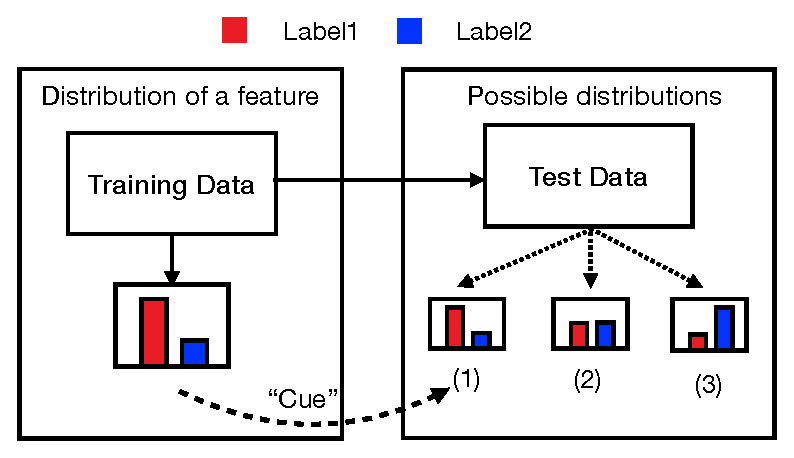
\includegraphics[width=0.6\columnwidth]{picture/cue_def.eps}
%\caption{Example of a {\em cue}. }
%%\KZ{``Possible distributions of the same feature''}}
%\label{fig:cue_def}
%\end{figure}

Previous studies~\cite{gururangan2018annotation,sanchez2018behavior,
poliak2018hypothesis} 
showed that linguistic features 
(e.g., sentiment, repetitive words and even shallow n-grams)
which are not essential in the reasoning processing but have
statistical correlation with specific labels in the data
can be the artifacts exploited by some machine learning models.
In this work, we call a linguistic feature an ``\textbf{extraneous feature}''
if it is not useful in determining the correct choice in a NLR question, 
and call an extraneous feature a ``\textbf{spurious cue}'' (or simply cue) if it strongly correlates 
with a particular type of label or choice in the dataset. 
Note that an extraneous feature is defined with respect to a single question or case,
while a cue is defined statistically.
Further, even if a cue exists in a dataset, a model trained on
it may or may not bias toward it. A model that is less susceptible to
spurious cues in the training data is a more robust model.
The goal of this work is develop an efficient framework that can do the following:
\begin{enumerate}[label=(\roman*)]
\item \textbf{identify extraneous features and spurious cues in any NLR dataset}; 
\item \textbf{test if a model trained on that dataset exploits an extraneous feature}; 
\item \textbf{explain why the model exploits that extraneous feature}.  
\end{enumerate}

To do (i), we first define a few types of linguistic features that are likely to be
introduced into the dataset as extraneous artifacts.
Given a question containing a certain feature, we develop an accurate classifier
that tells us if that feature is extraneous in the context by leveraging
a large pretrained language model.
If the feature is extraneous, its ``cueness'' can then be computed using a variety of
statistical measures, which will be evaluated in this paper. 

To do (ii), we develop a simple method to automatically neutralize the 
extraneous feature in a question without disturbing its logical
structure and thus create a new stress test question. A model $M$ is
considered exploiting the feature in the original question
if it changes its prediction on the stress test question.

To do (iii), we further stress test the original pretrain language model of $M$ 
without fine-tuning to see if the original PLM already show weakness on
that extraneous feature or if the weakness is developed while fine-tuning
on the training data which contains that feature as a cue.

%If the dataset contains reasonably sized test set, we propose 
%another metric to estimate a model's statstical bias toward a spurious linguistic
%feature in the test set. However, due to the statistical nature of
%this metric, it does not work well if the test set is not big enough.
%So we further propose a method to verify a model's sensitivity toward a
%spurious feature in a single problem instance. This provides
%microscopic evidence about a model's bias, which can be aggregated
%by a set of instances with the same feature.
We call this framework ICQ (I-See-Cue). We believe that
this framework will be useful to validate future models and
datasets in NLR research and its interpretation power can help
NLP practitioners to decide the robustness of a given model and
the reliability of their training data. 

%In this paper, our view is that the existing test sets for these
%tasks are not sufficiently exploited. Why do we go the extra mile to
%generate new test cases which are potentially incorrect, when we can
%test the models using existing test sets but from different perspectives?
%With this objective in mind, we propose an algorithm to statistically 
%determine possible biases that exist in a dataset.
%evaluating both the dataset and the corresponding models. In this framework, 
%one test dataset can be seen as multiple test sets from different perspectives. 
%which
%In this paper, we propose a light-weight framework called
%can evaluate both the {\em data set} and the {\em model} for
%discriminative NLI tasks {\em fully} automatically. 

%We illustrate this in~\figref{fig:cue_def}. 
%Once these cues are neutralized from the test data, 
%previously successful models may degrade substantially
%on it, suggesting that the model has taken advantage of 
%the biased feature and is hence not as robust as assumed 
%against with such cues.

%Inspired by the black-box testing in CheckList, 
%%whwith various of perturbation strategies, like typos, 
%we propose to generate test cases by just 
%filtering the original test data into new subsets according to 
%specific linquistic features, like word, NER, Negation, and sentiment, etc. 
%%in constructing the spurious cues. 
%We can show the cases distribution on each label indicates whether 
%the dataset is balance on this feature. In another word, we can 
%find the bias and cues intuitively. 
%Meanwhile,  we can prob what bias features the model really sensitive to.
%We even out the filtered test date on different labels. The even out version 
%can be used as a ``feature test'' to estimate whether a model consider 
%bias features in training data to make prediction.
%
%Our framework can be used to identify simple but effective biases and cues  
%in a broad range of multiple choice NL reasoning datasets.
%Though not all multiple choice questions in these dataset involve 
%all three components, i.e., a premise, a hypothesis and a label, 
%we will describe in~\secref{sec:formulation} how to normalize them into
%the standard form. 

%The relative size of hard part over the whole
%data indicates the quality of the dataset .
%\KZ{pls quickly finish the remaining part of intro. 
%The contributions part is critical.}
%Thus we can
%separate the original dataset into easy and hard part with 
%the bias score feature of cues
%any   dataset into easy and hard part
%and thus we can evaluate the ``biasness'' and ``quality'' of the dataset. 

%using simple and cost-effective linear classification models 
%on the simple cue features,
%which trained with unbalanced score of cues to several benchmark datasets across 
%various tasks and domains. 
%We evaluate the effectiveness of our methods with the 
%deviation between our results and random selection results. 
%Simultaneously, the test set can be divided into two parts: \textbf{easy} and \textbf{hard}. 
 %\textbf{balance} and \textbf{imbalance} are relative rather than absolute. 
%\KZ{Improving the neural models by splitting the training set.} 

%The training data can be separated into $n$ parts, test on one part and training 
%the model on the rest for each time. 
%The filtered part contains the instances 
%which can not be correctly chosen.
%The filtered data will be used to train a better model for target tasks. 

In summary, this paper makes the following contributions:
%\KZ{These contribs need to be revised right?}
\begin{itemize}
\item we propose and implement ICQ, a novel framework for detecting
the linguistic artifacts in NLR datasets and as well as weakness
in deep models against these artifacts;

\item using ICQ, for the first time, 
we are able to not only pinpint the exact linguistic feature that
an NLR model is ``cheating'' on when answering a question,
but also explain why the model is susceptible to this feature.
%(\secref{sec:result}).

%\item we propose a simple blackbox test to quantitatively 
%assess whether a given model has taken advantage of a
%statistical cue globally (\KZ{Note even if the model exploit a cue
%strongly, the cue may not be spurious!});

%\item we develop both manual and automatic methods to perturb a spurious
%feature in a problem instance, and show that these methods can be used to
%effectively test the model's weakness on the feature.

\item our comprehensive evaluation of ICQ on 4 popular NLR datasets and 
3 models shows that XXX is more robust than YYY despite that the ZZZ dataset
contains many cues; and that YYY picked up some biases from the pretrain data. 
We speculate that the pretrain data ...
%\item we created an online demonstration system to showcase
%the results and invite users to evaluate their own datasets and models.
\end{itemize}
% (\secref{sec:result}).

%\item We filter the training data and get a better performance on the \textbf{hard} dataset.
%to get a high quality training dataset which
 %is possibly closer to the intended task. 

